
\subsection{nanoGPT Speedrunning}


\begin{wraptable}{r}{0.47\textwidth}
        \centering
        \vspace{-10pt}
        \caption{Perplexity for \algname{} and Muon on Qwen2-0.5B pre-training.}
        \label{tab:qwen2-0.5B}
        \begin{tabular}{l cc cc}
            \toprule
            $\eta$ &
            \multicolumn{2}{c}{\algname{}} &
            \multicolumn{2}{c}{Muon} \\
            \cmidrule(lr){2-3}\cmidrule(lr){4-5} 
            & \multicolumn{2}{c}{$\lambda=0.0$} 
            & $\lambda=0.1$ & $\lambda=0.0$  \\
            \midrule
            $1\times 10^{-2}$   & \multicolumn{2}{c}{$14.57$} & -- &  -- \\
            $8\times 10^{-3}$   & \multicolumn{2}{c}{$14.59$} & $46.77$ & $94.02$ \\
            $4\times 10^{-3}$   & \multicolumn{2}{c}{$14.65$} & $14.86$ & $14.83$ \\
            $2\times 10^{-3}$   & \multicolumn{2}{c}{$14.76$} & $14.82$ & $14.88$ \\
            $1\times 10^{-3}$   & \multicolumn{2}{c}{$14.95$} & $14.91$ & $15.03$ \\
            \bottomrule
        \end{tabular}%
        
    \vspace{-20pt}
\end{wraptable}


We compare \algname{} and Muon for different learning rates and widths using the \texttt{modded-nanoGPT} codebase and report the results in Fig.~\ref{fig:modded-nanogpt-learning-rate}. Similar to \cite{pethick_training_2025}, we choose a log-space learning grid from $2^{-12}$ to $2^{-5}$. Fig.\ \ref{fig:modded-nanogpt-learning-rate} confirms the conclusions drawn in the main text regarding the greater robustness with respect to ill-chosen learning rates. 

\begin{figure}
    \centering
    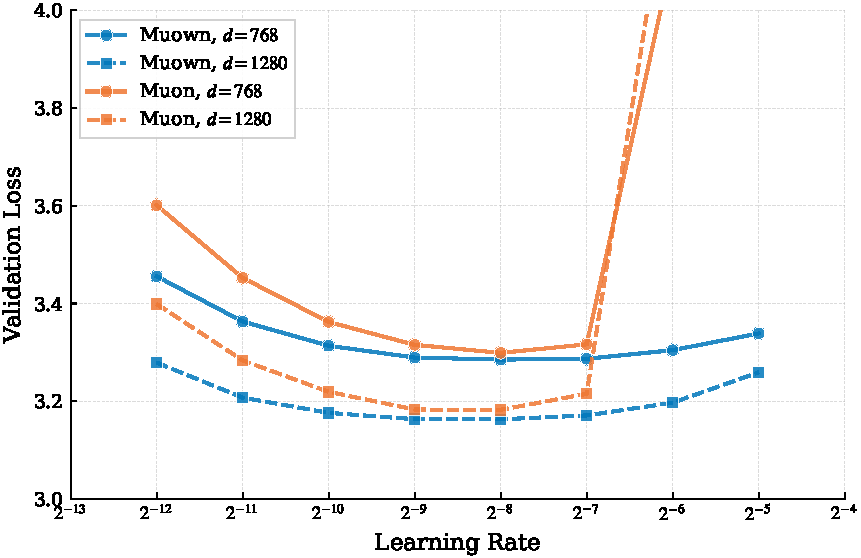
\includegraphics[width=0.5\linewidth]{figures/experiment_modded_nanogpt_run.pdf}
    \caption{Learning rate and width ablation for Muon and \algname{} using the \texttt{modded-nanoGPT} codebase. }
    \label{fig:modded-nanogpt-learning-rate}
\end{figure}

\subsection{Qwen2-0.5B}
\label{sec:qwen2-exp}

As an additional architectural datapoint, we pre-train a Qwen2-0.5B \citep{yang_qwen2_2024} model, reporting results in Table~\ref{tab:qwen2-0.5B}. We remark that for all but one learning rate considered, \algname{} outperforms Muon and maintains a 0.25 perplexity advantage when comparing the best-performing hyperparameters. 


\subsection{Comparison with NorMuon}
\label{appdx:normuon-comparison}

\begin{wrapfigure}{r}{0.5\textwidth}
    % \vspace{-10pt}
    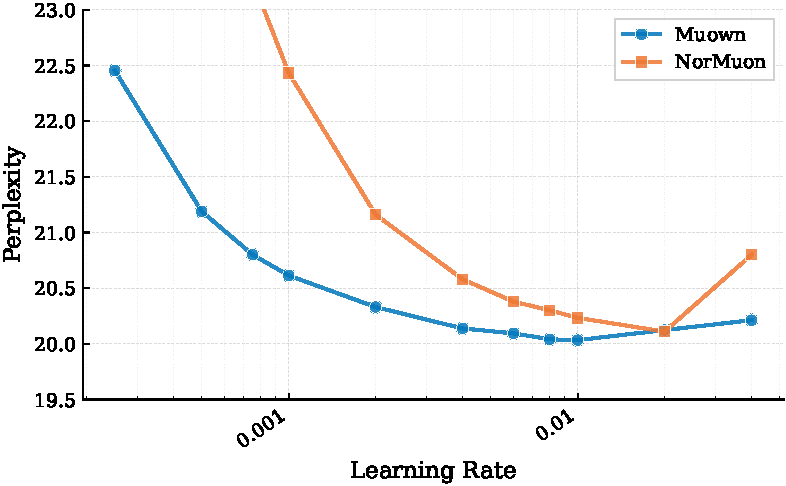
\includegraphics[width=0.5\textwidth]{figures/experiment_normuown/lr_ablation_perplexity_wd_False.pdf}
    \caption{Comparison of NorMuon and \algname{} on a 124M model.}
    \vspace{-10pt}
    \label{fig:normuon-comparison}
\end{wrapfigure}
Both NorMuon \citep{li_normuon_2025} and Muown augment plain Muon with a per-row mechanism on the rows of the 2D weight matrices, but they intervene at different points in the update. Plain Muon orthogonalizes the momentum of $\nabla_\W \mathcal{L}$ via Newton–Schulz and applies it directly to the parameter without a row-wise state. NorMuon instead applies a post-processing step to the update, maintaining a per-row EMA of the mean-squared entries of the orthogonalized update, dividing the update element-wise by its square root, and renormalizing back to the original Frobenius norm. This procedure effectively redistributes mass of the update across rows. In contrast, rather than redistributing mass of the update \algname{} changes the parameterization to control the row-norms of the weight. In essence, both methods equip every row with a scalar quantity (a second-moment statistic for NorMuon and a learned magnitude for \algname{}). Nevertheless, these row variables serve different purposes. We compare both methods on a 124M model across eleven learning rates spanning $2.5 \times 10^{-4}$ to $4 \times 10^{-2}$. Muown matches or improves on NorMuon at most learning rates that lie near the optimum and exhibits a noticeably wider basin of stability.

\subsection{Spectral Analysis}
\label{appdx:spectral-experiments}

We provide more detailed results for the empirical association between $\norm{\W_t}_2^2$ and $\norm{\g_t}_\infty$. Figs.~\ref{fig:spectral-norm-detailed}, \ref{fig:row-norm-detailed}, and \ref{fig:lambda-max-detailed}, show the evolution of $\norm{\W_t}_2^2$, $\norm{\g_t}_\infty$, and $\lambda_{\max}(\PP_t\,\C_t\,\PP_t)$, respectively. Each row depicts the quantities mentioned above computed on the weights of a transformer block of a 500M model trained with either of Muon and \algname{}. We remark that for all layers and weight types considered the spectral norm and maximal row norm are moving in lock step, while $\lambda_{\max}(\PP_t\,\C_t\,\PP_t)$ remains bounded.

Moreover, we provide more detailed results on the spectral distribution of the layers in the 16th transformer block in Figs.~\ref{fig:spectral-analysis-detailed}, \ref{fig:spectral-histogram-detailed}, and \ref{fig:spectral-distribution-lineplot}. 



\begin{figure}
    \centering
    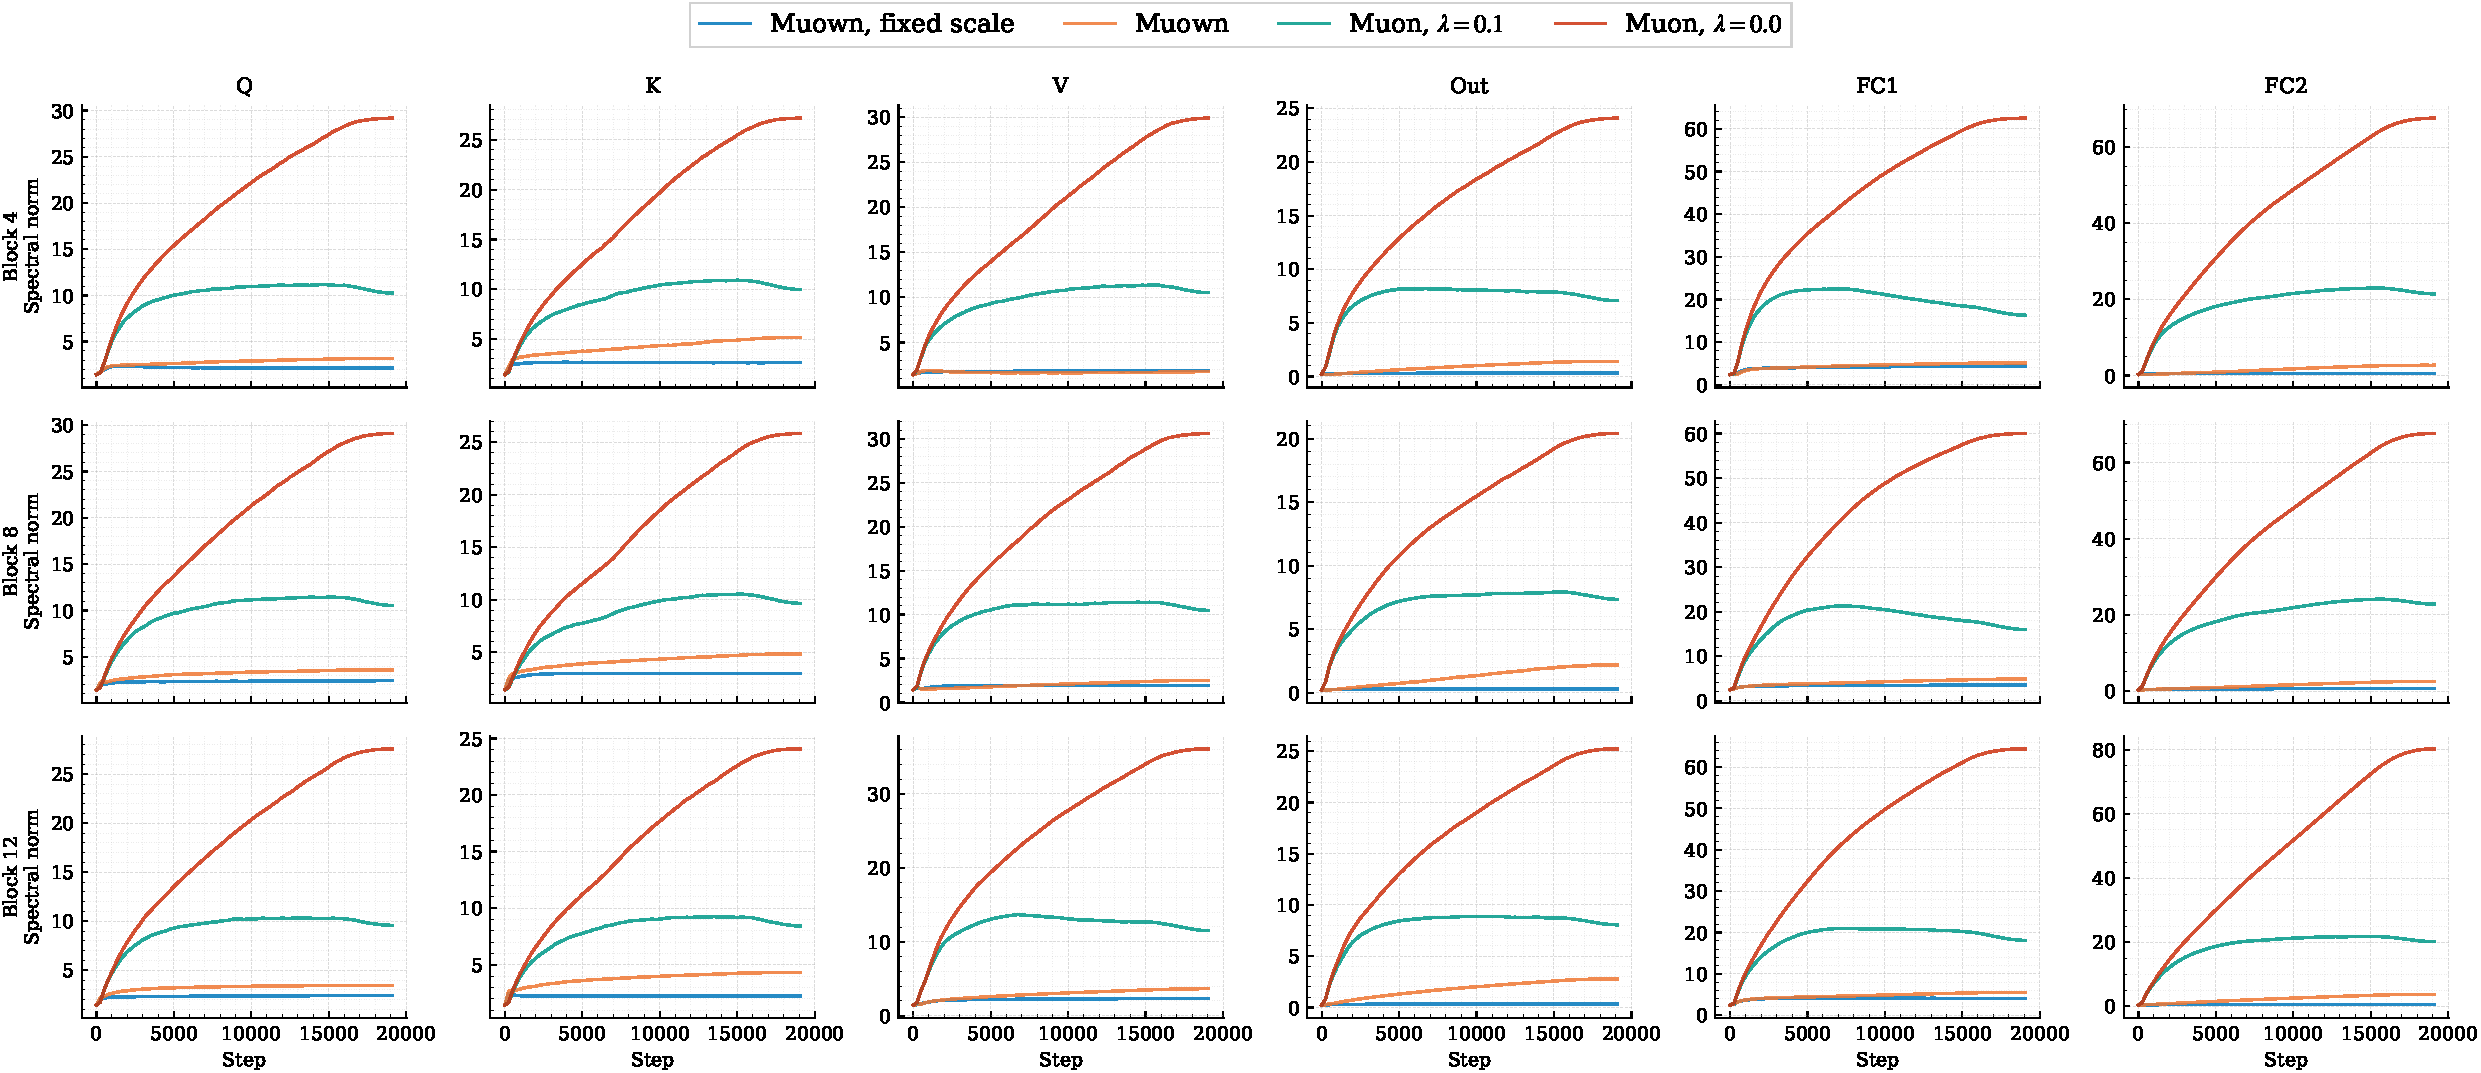
\includegraphics[width=\linewidth]{figures/experiment_magnitude_optim_ablation/spectral_norm_grid.pdf}
    \caption{$\opnorm{\W_t}$ for the layers in the 4th, 8th, and 12th transformer block of a 500M model.}
    \label{fig:spectral-norm-detailed}
\end{figure}

\begin{figure}
    \centering
    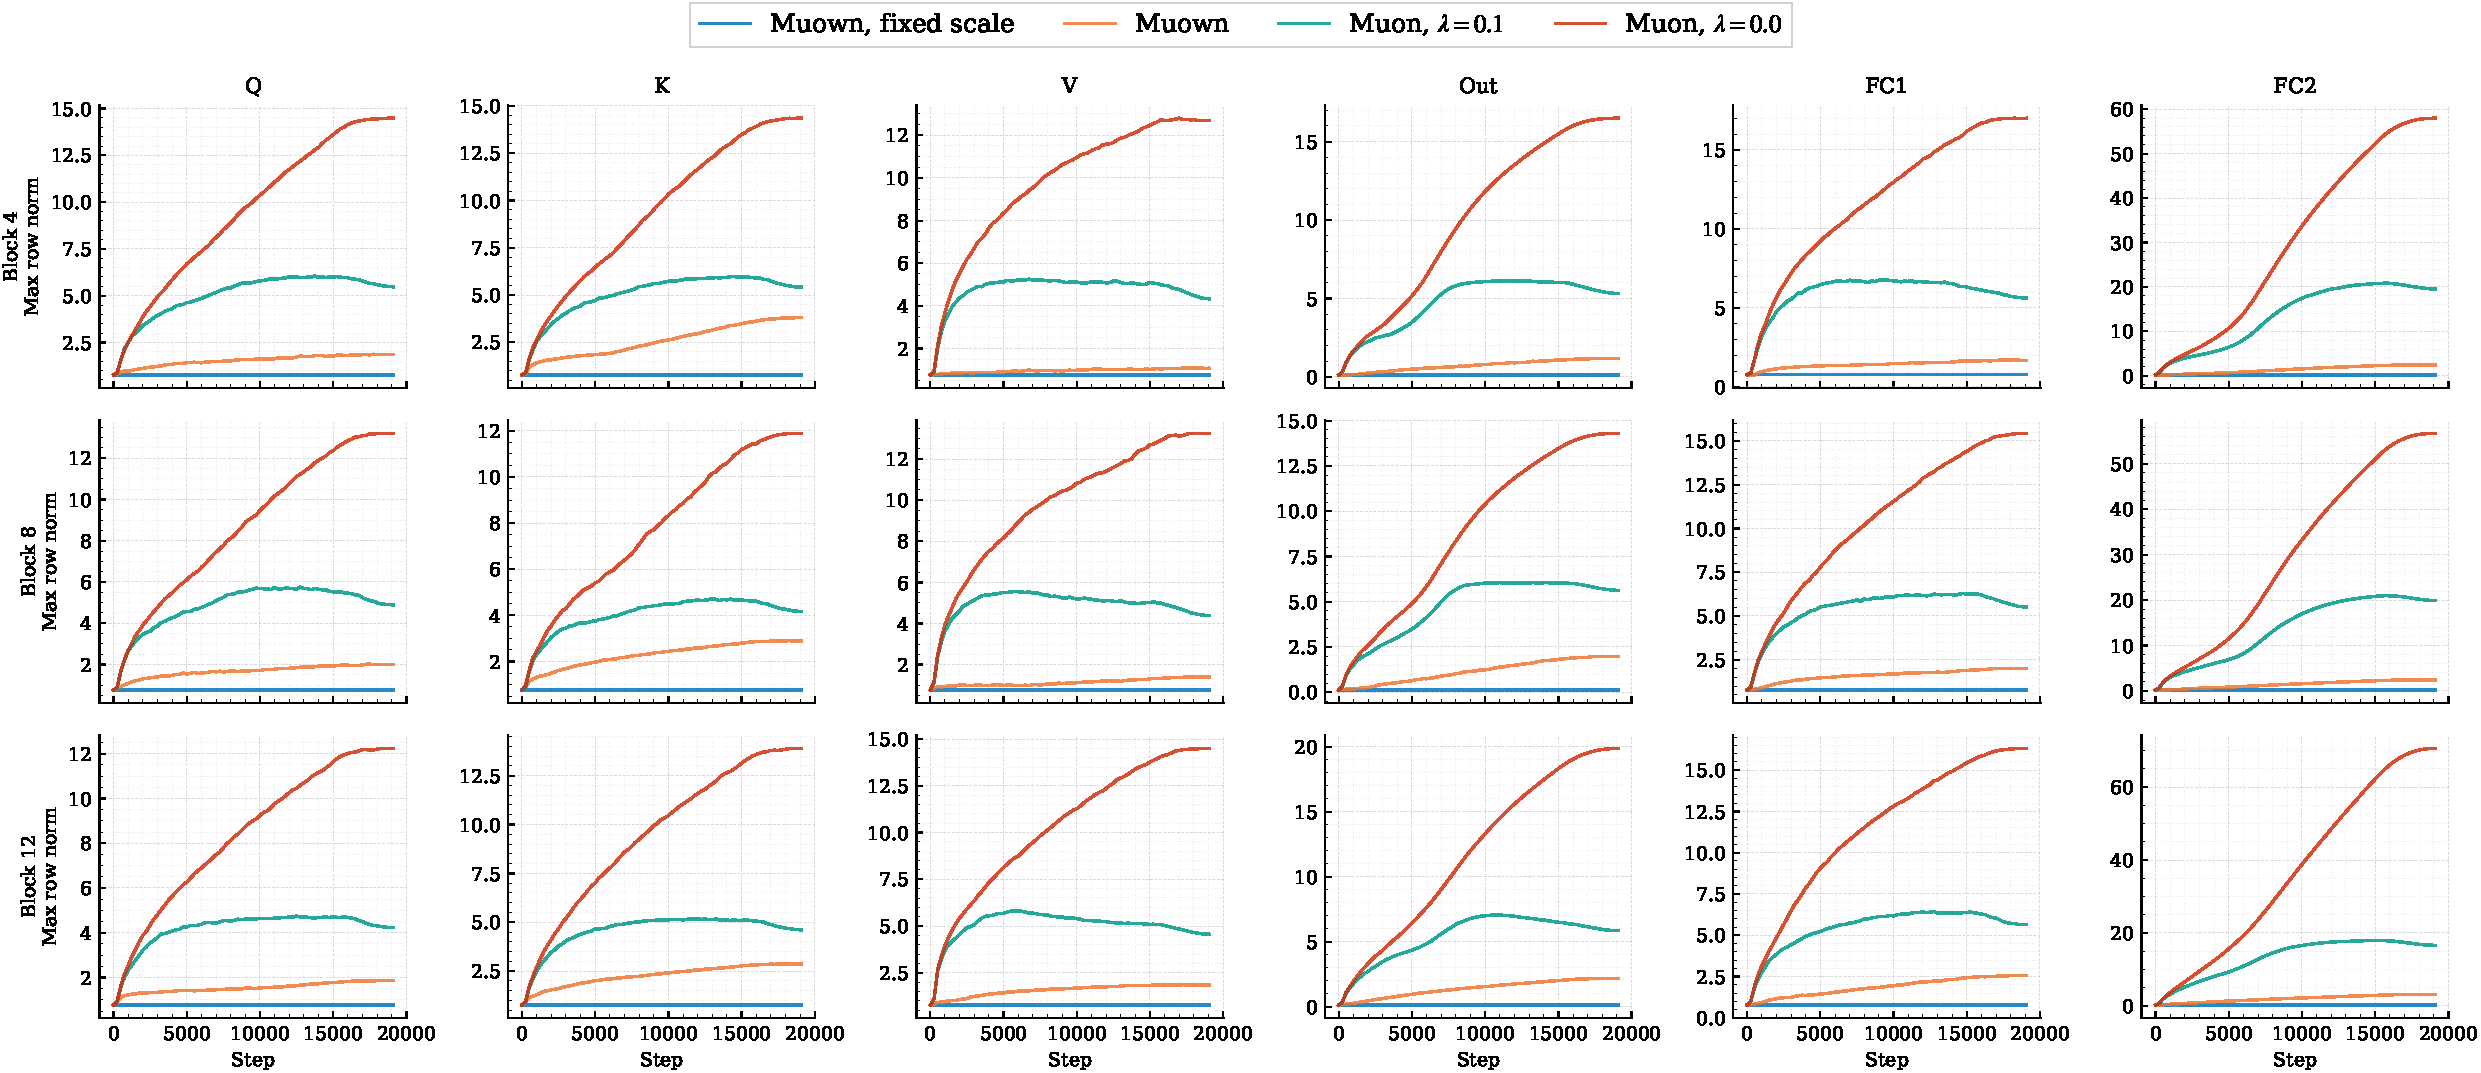
\includegraphics[width=\linewidth]{figures/experiment_magnitude_optim_ablation/max_row_norm_grid.pdf}
    \caption{$\norm{\g_t}_\infty$ for the layers in the 4th, 8th, and 12th transformer block of a 500M model.}
    \label{fig:row-norm-detailed}
\end{figure}


\begin{figure}
    \centering
    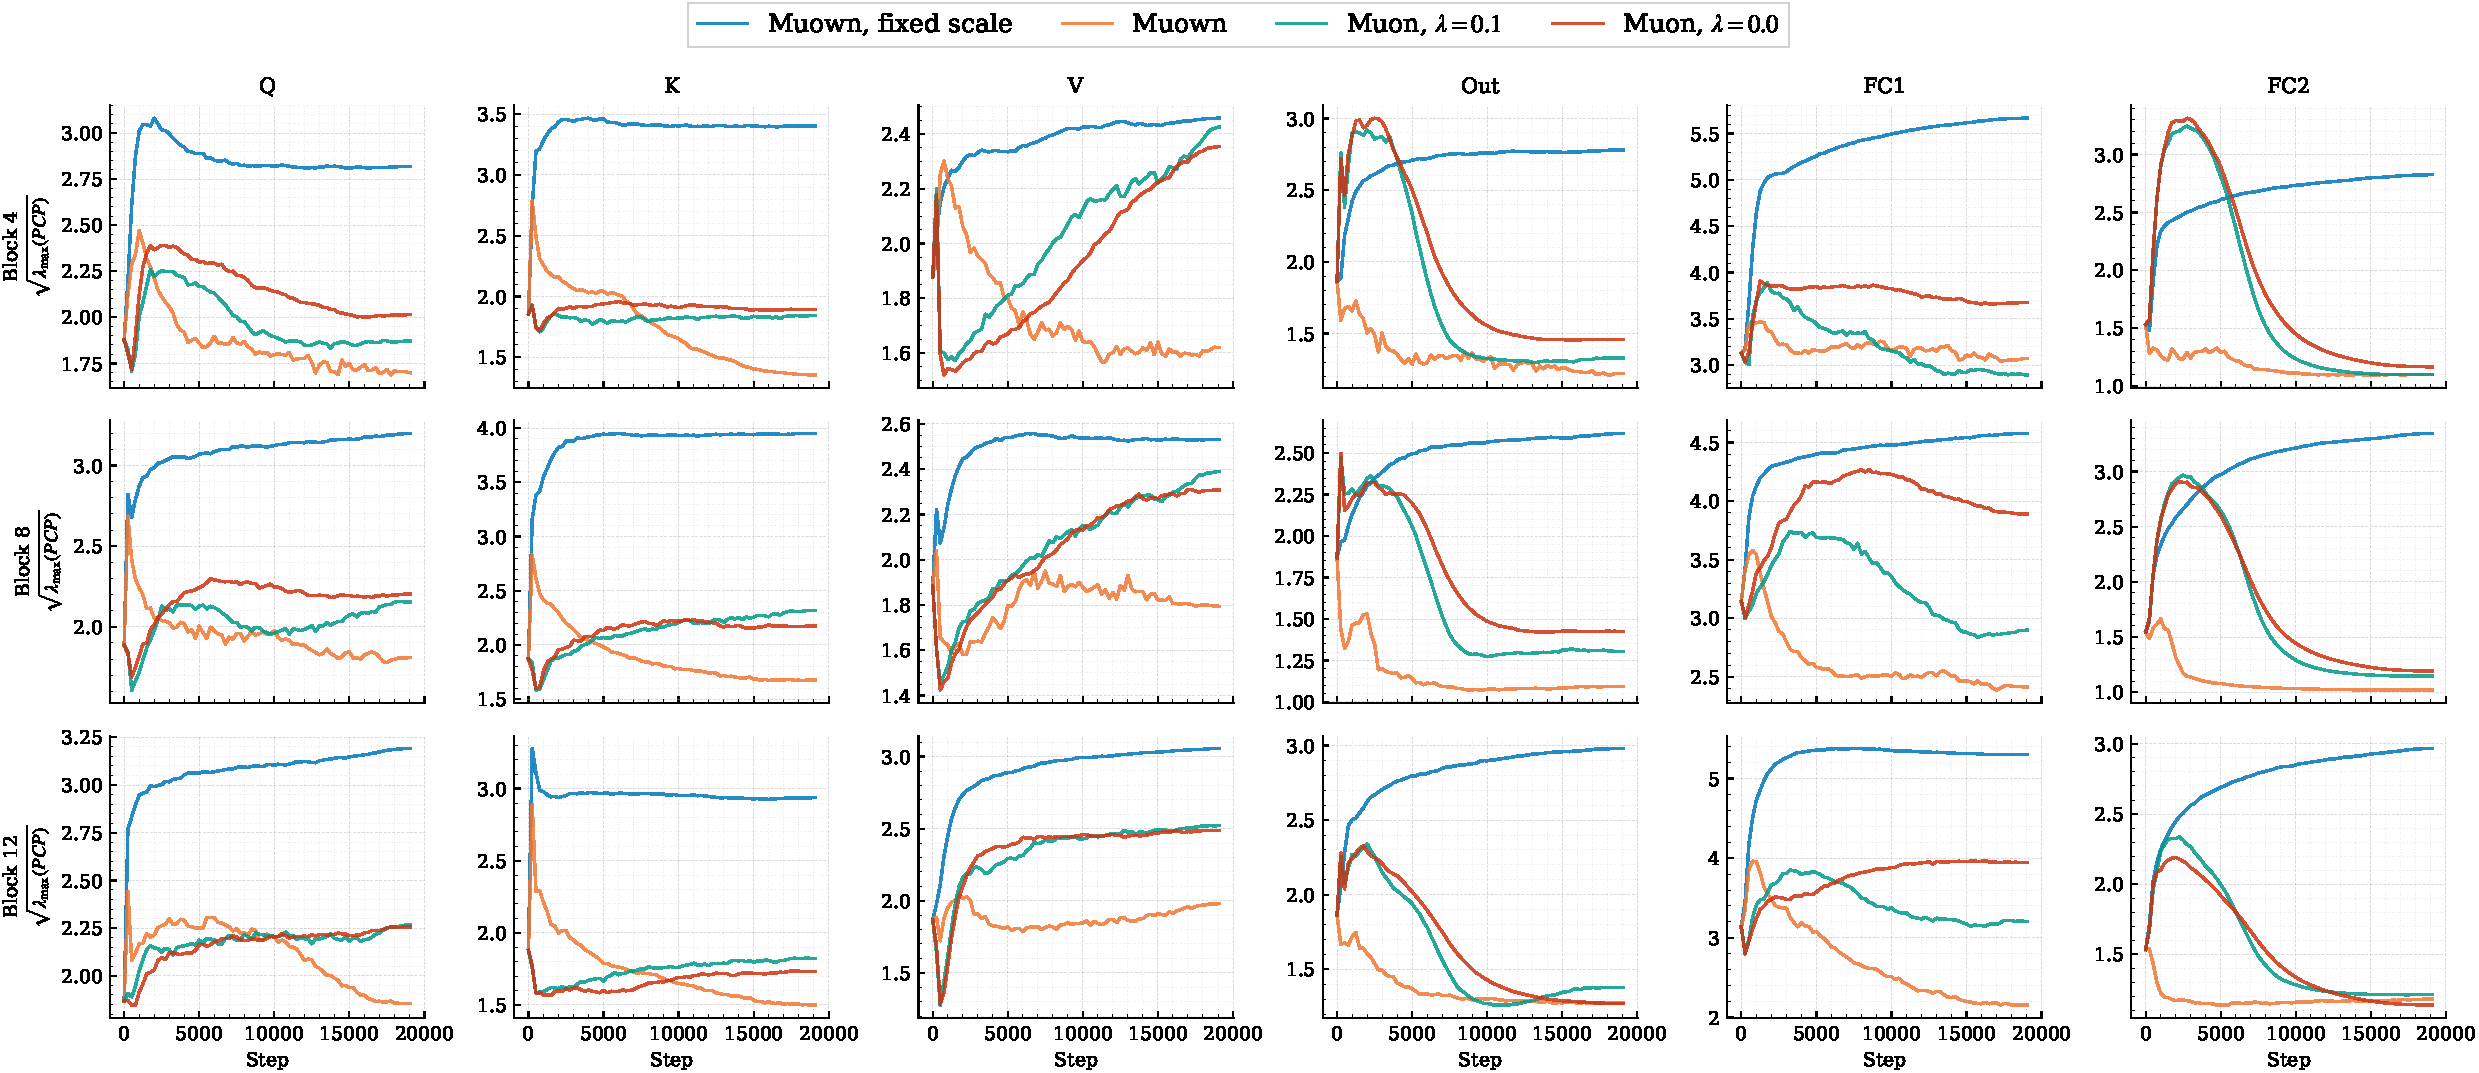
\includegraphics[width=\linewidth]{figures/experiment_magnitude_optim_ablation/lambda_max_PCP_grid.pdf}
    \caption{$\sqrt{\lambda_{\max}(\PP_t\,\C_t\,\PP_t)}$ for the layers in the 4th, 8th, and 12th transformer block of a 500M model.}
    \label{fig:lambda-max-detailed}
\end{figure}



\begin{figure}[t]
    \centering
    \begin{subfigure}[t]{0.245\textwidth}
        \centering
        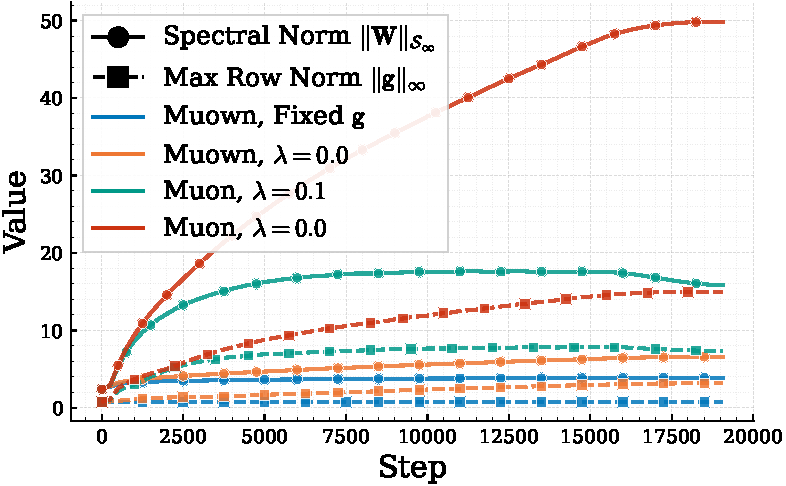
\includegraphics[width=\textwidth]{figures/experiment_magnitude_optim_ablation/0506_spectral_norm_max_row_norm_layers_16_mlp_fc1_weight.pdf}
        \caption{MLP Layer 1}
        \label{fig:spectral-analysis-detailed-mlp1}
    \end{subfigure}\hfill
    \begin{subfigure}[t]{0.245\textwidth}
        \centering
        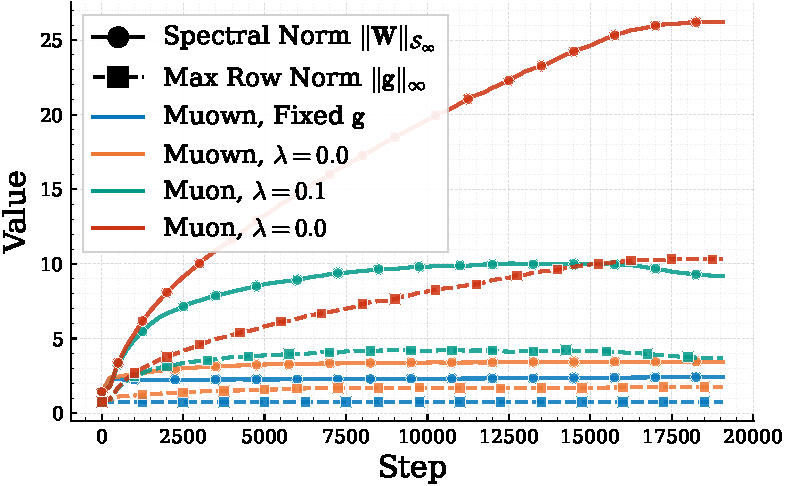
\includegraphics[width=\textwidth]{figures/experiment_magnitude_optim_ablation/0506_spectral_norm_max_row_norm_layers_16_attn_w_q_weight.pdf}
        \caption{Query Projection}
    \end{subfigure}\hfill
    \begin{subfigure}[t]{0.245\textwidth}
        \centering
        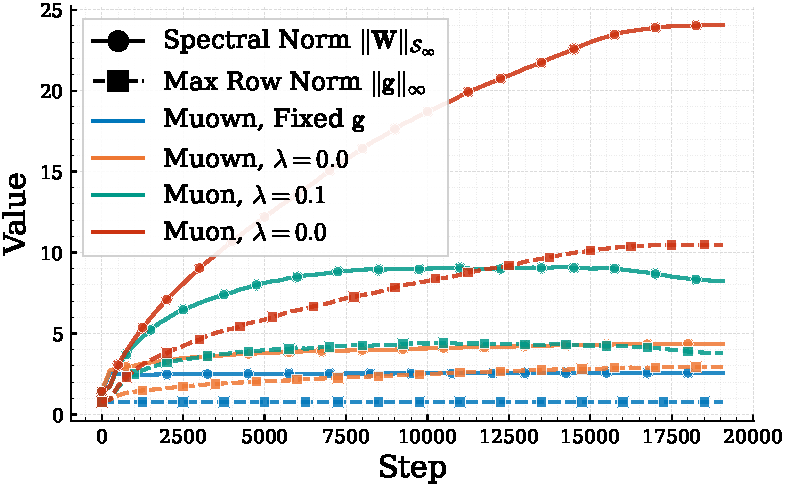
\includegraphics[width=\textwidth]{figures/experiment_magnitude_optim_ablation/0506_spectral_norm_max_row_norm_layers_16_attn_w_k_weight.pdf}
        \caption{Key Projection}
    \end{subfigure}
    \begin{subfigure}[t]{0.245\textwidth}
        \centering
        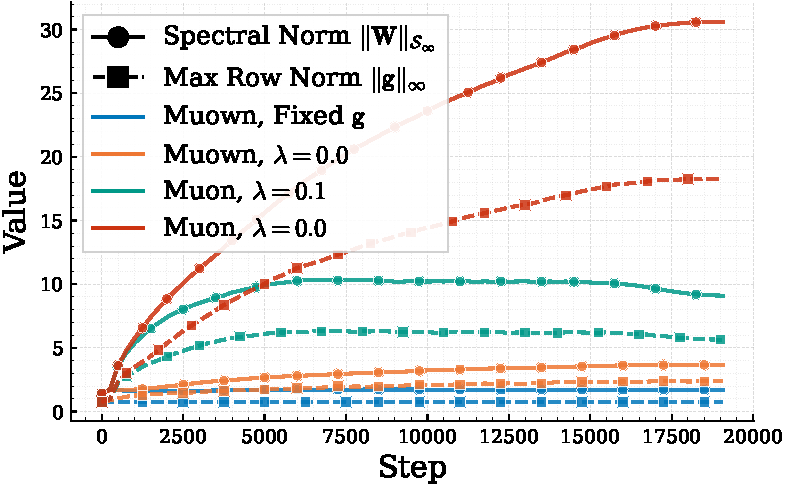
\includegraphics[width=\textwidth]{figures/experiment_magnitude_optim_ablation/0506_spectral_norm_max_row_norm_layers_16_attn_w_v_weight.pdf}
        \caption{Value Projection}
    \end{subfigure}

    \caption{Evolution of spectral norm $\opnorm{\W_t}$ and maximum row norm $\|\g_t\|_{\infty}$ over the course of training for linear layers of the 16th transformer block of a 500M model. }
    \label{fig:spectral-analysis-detailed}
\end{figure}



\begin{figure}[t]
    \centering
    \begin{subfigure}[t]{0.245\textwidth}
        \centering
        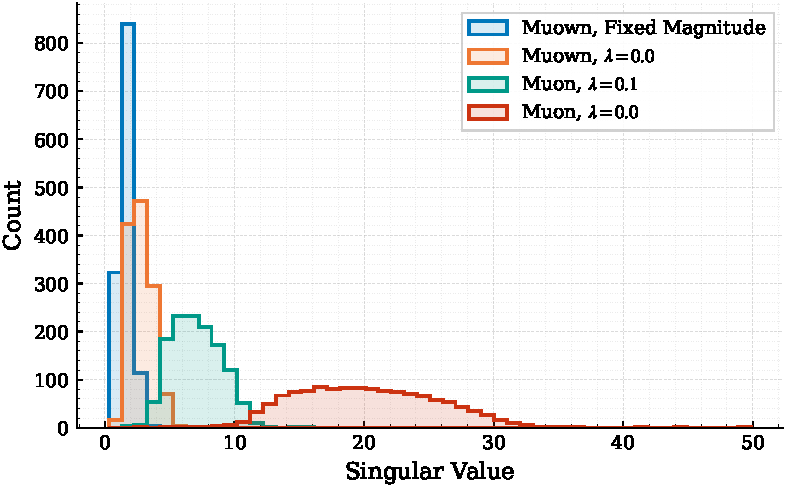
\includegraphics[width=\textwidth]{figures/experiment_magnitude_optim_ablation/sv_hist_layers_16_mlp_fc1.pdf}
        \caption{MLP Layer 1}
    
    \end{subfigure}\hfill
    \begin{subfigure}[t]{0.245\textwidth}
        \centering
        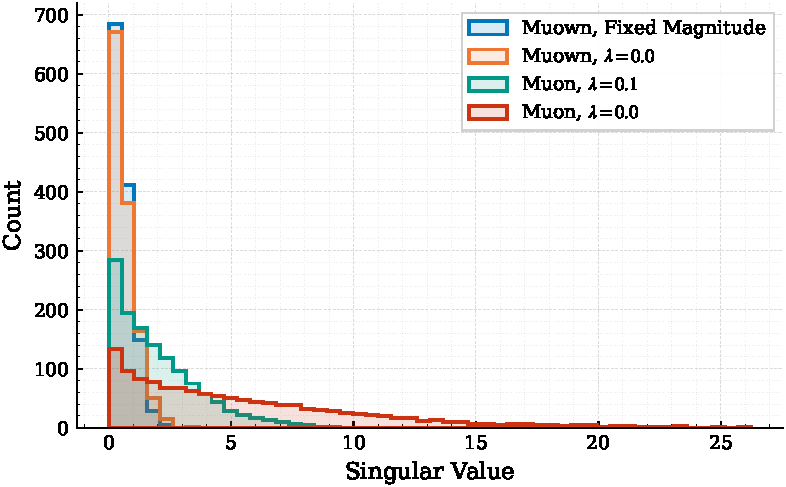
\includegraphics[width=\textwidth]{figures/experiment_magnitude_optim_ablation/sv_hist_layers_16_attn_w_q.pdf}
        \caption{Query Projection}
    \end{subfigure}\hfill
    \begin{subfigure}[t]{0.245\textwidth}
        \centering
        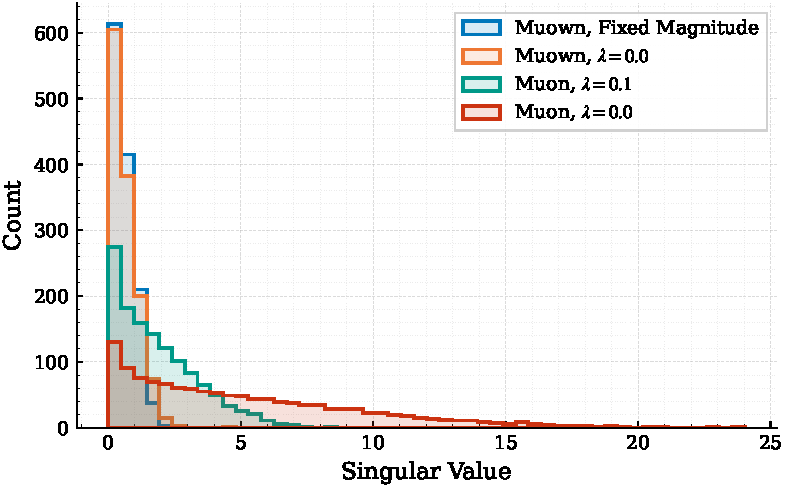
\includegraphics[width=\textwidth]{figures/experiment_magnitude_optim_ablation/sv_hist_layers_16_attn_w_k.pdf}
        \caption{Key Projection}
    \end{subfigure}
    \begin{subfigure}[t]{0.245\textwidth}
        \centering
        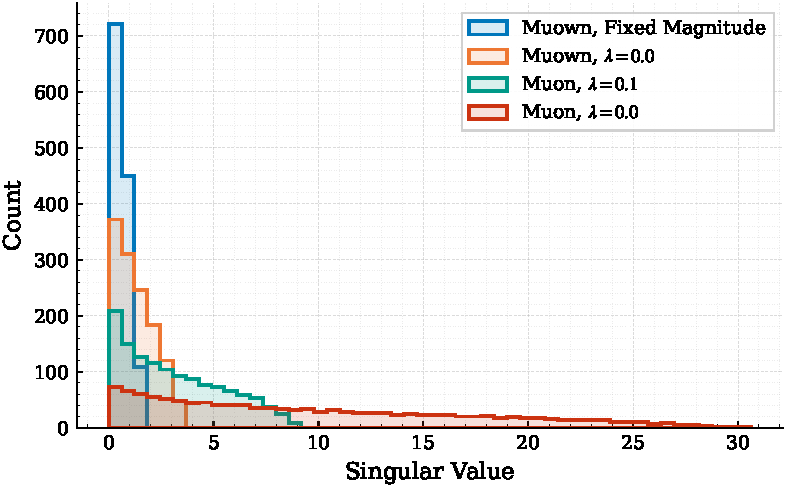
\includegraphics[width=\textwidth]{figures/experiment_magnitude_optim_ablation/sv_hist_layers_16_attn_w_v.pdf}
        \caption{Value Projection}
    \end{subfigure}
        
    \caption{Histogram of singular values for linear layers of the 16th transformer block of a 500M model.}
    \label{fig:spectral-histogram-detailed}
\end{figure}



\begin{figure}
    \centering
    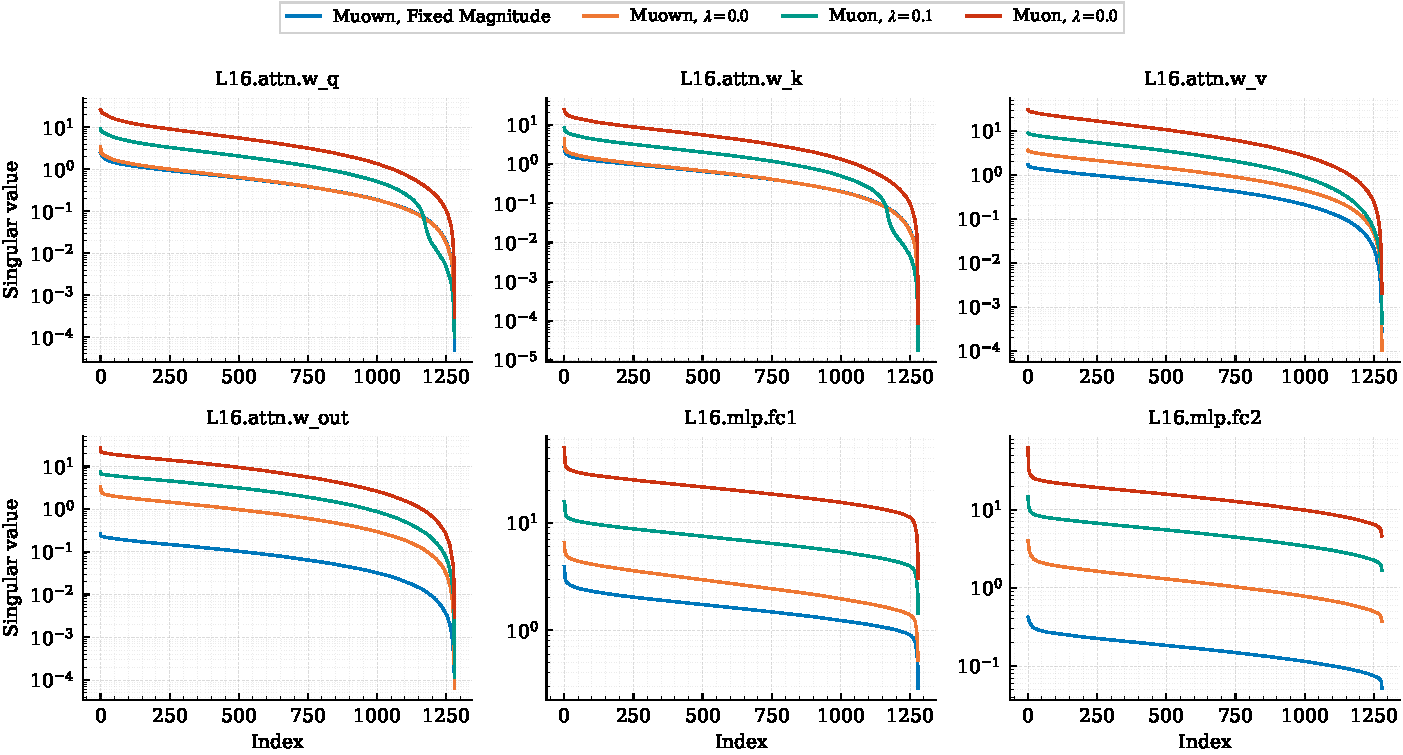
\includegraphics[width=\linewidth]{figures/experiment_magnitude_optim_ablation/sv_lineplot_16_logscale_True.pdf}
    \caption{Singular value distribution for linear layers of the 16th transformer block of a 500M model. \texttt{attn} refers to the attention block with \texttt{w\_q}, \texttt{w\_k}, \texttt{w\_v}, \texttt{w\_out} denoting query, key, value, and output projections, respectively. \texttt{fc1} and \texttt{fc2} refer to the first and second MLP layers of the block.}
    \label{fig:spectral-distribution-lineplot}
\end{figure}


\subsection{Magnitude Learning}
\label{appdx:magnitude-learning}

In Section~\ref{sec:motivation}, we identify $\|\g_t\|_\infty$ as the empirical driver of $\opnorm{\W_t}$ drift under Muon and remark that freezing $\g_t = \g_1$ at initialization eliminates the systematic growth in spectral norm. Nevertheless, it remains open how effective such a strategy is in terms of perplexity. As Table~\ref{tab:magnitude-optimizer} demonstrates empirically, suppressing row-norm growth alone already accounts for a significant part of the improvement over Muon: \emph{Fixed}, which freezes row magnitudes at initialization, outperforms Muon at the smaller learning rates and prevents the divergence at $\eta = 4 \times 10^{-3}$ (Table~\ref{tab:magnitude-optimizer}), without learning the magnitudes. Training $\g$ on top, with either of SignSGD+Momentum (Signum) or Adam, refines the result further, with the ordering between Adam, Signum, and Fixed preserved across all three learning rates. While we find the \emph{Fixed} variant to perform slightly worse than the ones with trainable magnitudes, it can serve as a more lightweight alternative that does not require storage of the Adam states and further simplifies the update procedure.

\begin{table}%{r}{0.5\textwidth}
        \vspace{-10pt}
        \centering
        \setlength{\tabcolsep}{4pt}
        \caption{Perplexity for \algname{} on a 500M model using different magnitude optimizer choices.}
        \label{tab:magnitude-optimizer}
        % \resizebox{\linewidth}{!}{%
        \begin{tabular}{l ccc}
            \toprule
            $\eta$ & \multicolumn{3}{c}{\algname{}} \\
            \cmidrule(lr){2-4}
             &  Fixed & Signum & Adam \\
            \midrule
            $4 \times 10^{-3}$ & 14.22 & 14.21 & 14.11 \\
            $2 \times 10^{-3}$ & 14.21 & 14.18 & 14.11 \\
            $1 \times 10^{-3}$ & 14.30 & 14.27 & 14.24 \\
            \bottomrule
        \end{tabular}%
        % }
\end{table}



\subsection{Effective Rank of Minibatch Gradients}
\label{appdx:effective-rank}

Combined with Fig.~\ref{fig:gradient-conditioning} in the main text, Fig.~\ref{fig:gradient-conditioning-remaining} covers all six linear weight types of the transformer block (queries, keys, values, output projection, and both MLP layers). The same pattern holds across types: \algname{} sustains a higher normalized effective rank than Muon throughout training on every weight type considered, with the gap opening early in training and persisting for the entire run. 



\begin{figure}[t]
        \centering
    \begin{subfigure}[t]{0.33\textwidth}
        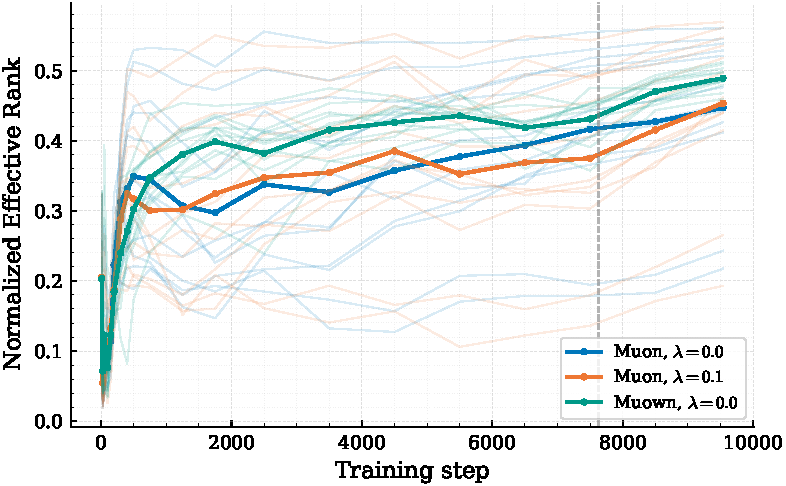
\includegraphics[width=\textwidth]{figures/experiment_gradient_conditioning/effective_rank_normalized_K.pdf}
        \caption{Key}
        \label{fig:eff-rank-w_k}
    \end{subfigure}
    \begin{subfigure}[t]{0.33\textwidth}
         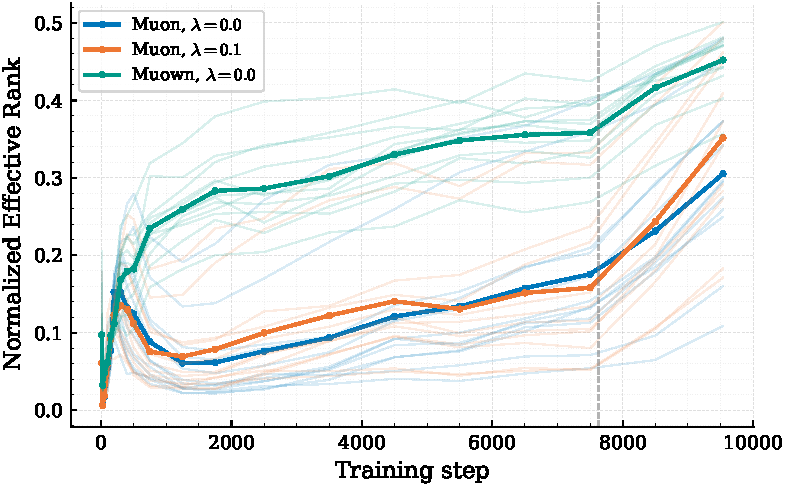
\includegraphics[width=\textwidth]{figures/experiment_gradient_conditioning/effective_rank_normalized_V.pdf}
         \caption{Value}
         \label{fig:eff-rank-w_v}
    \end{subfigure}\hfill
    \begin{subfigure}[t]{0.33\textwidth}
         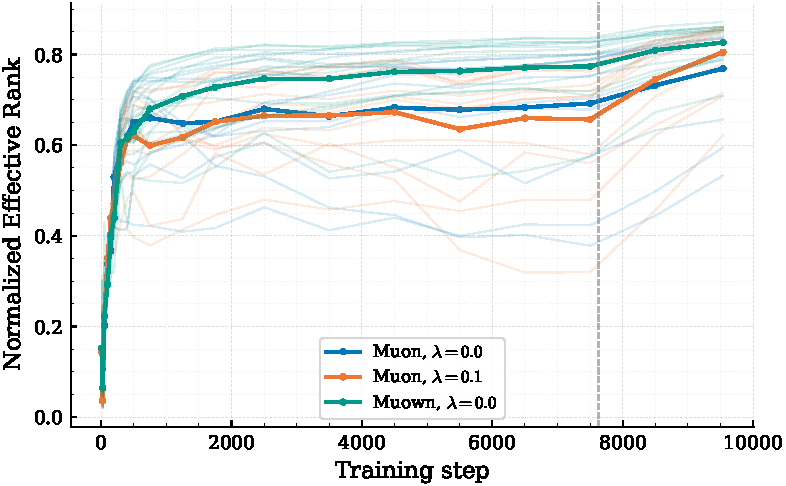
\includegraphics[width=\textwidth]{figures/experiment_gradient_conditioning/effective_rank_normalized_fc2.pdf}
         \caption{MLP Layer 2}
         \label{fig:eff-rank-fc2}
    \end{subfigure}\hfill

    \caption{Normalized effective rank \citep{roy_effective_2007} of minibatch gradients for a 124M model. At a given training step, we sample 8 gradients and average their effective ranks.}
    \label{fig:gradient-conditioning-remaining}
    % \vspace{-20pt}
\end{figure}
